\newpage
\restoregeometry
\section{Grundlagen}
\subsection{Radarfernerkundung}
Bei der Radarfernerkundung werden vom Radarsystem in regelmäßigen Abständen elektromagnetische Signale ausgesandt. Nach dem Senden eines Signals 
(Chrip) folgt ein Zeitfenster indem die Plattform auf Echos des ausgesandten Signals wartet.
Trifft das ausgesandte Signal auf eine Oberfläche, zum Beispiel 
die Erdoberfläche, wird ein Bruchteil reflektiert und als Echo vom Fernerkundungssystem empfangen \cite{tutorial_on_sar}.

Die Radarfernerkundung gehört zu den aktiven Fernerkundungsmethoden da hier im Gegensatz zur optischen Fernerkundung nicht nur 
von Oberflächen reflektierte Strahlung von anderen Strahlungsquellen wie der Sonne aufgenommen wird, sondern das Fernerkundungssystem 
selbst als Strahlungsquelle dient. Messungen können daher tageszeitunabhängig erfolgen. Dabei können die sendenden und erfangenden Komponenten 
unterschiedlich (bi- oder multistatisches Radar) oder identisch sein (monostatitsches Radar). Bildgebende Radarsysteme werden auf mobilen Plattformen 
montiert und blicken seitlich auf die zu beobachtende Oberfläche. Die Flugrichtung wird Azimut und die Blickrichtung als Slant Range bezeichnet. 

Die Eigenschaften des reflektierten Signals hängen sowohl von Parametern des Aufnahmesystems als von Parametern der reflektierenden Oberfläche ab.
So werden in der Radarfernerkundung verschiedenen Frequenzbänder verwendet, welche sich in Frequenz und Wellenlänge unterscheiden. (Warum?) 
Mit einer größeren Wellenlänge kann ein Medium tiefer durchdrungen werden. Außerdem werden Wolken, Dunst und Rauch durchdrungen was den zusätzlich Vorteil bietet
wetterunabhängig Messungen durchführen zu können \cite{einfuehrung_in_fernerkundung}.

\begin{table}[htb]
    \caption{Gängige Frequenz-Bänder in der Radarfernerkundung}
\begin{center}
    \begin{tabular}{|c|c|c|c|c|c|c|c|} 
        Frequenzband & Ka & Ku & X & C & S & L & P\\ 
        \hline
        Frequenz (GHz) & 40-25 & 17.6-12 & 12-7.5 & 7.5-3.75 & 3.75-2 & 2-1 & 0.5-0.25\\ 
        Wellenlänge (cm) & 0.75–1.2 & 1.7–2.5 & 2.5–4 & 4–8 & 8–15 & 15–30 & 60–120\\ 
    \end{tabular}
    \label{table:1}
\end{center}
    \text{Quelle: }
\end{table}

Die Durchdringungstiefe hängt auch von der Dielektrizitätskonstante der reflektierenden Oberfläche ab. Ist diese groß, reflektiert die Oberfläche stark und die 
Durchdringungstiefe ist gering. Zusätzlich ist die Polarisation der ausgesandten und empfangenen Signale bei der Messung ausschlaggebend. Sie können horizontal oder 
vertikal polarisiert sein. Dies führt zu vier möglichen Polarisationsmodi für das Senden (transcieve) und das Empfangen (receive) nämlich HH, VV, HV und VH.

Die Auflösung entlang des Azimut unterscheidet sich von der Auflösung in Blickrichtung. Die Auflösung in Azimutrichtung wird von der Antennenlänge 
bestimmt da diese festlegt wie lange die Reflektion eines Objektes empfangen werden. Die Antennenlänge kann bauartbedingt nicht beliebig gesteigert werden.
Die Antennenlänge bestimmt auch den Abstrahlwinkel und somit die Ausdehnung am Boden eines Impulses in Azimutrichtung. Diese nimmt mit zunehmender Entfernung
zu, während die Auflösung abnimmt.

Die Auflösung in Blickrichtung hängt vom Depressionswinkel der Antenne ab da dieser Einfluss auf die Laufzeit des Signals nimmt. Die Ausdehnung des beobachteten Gebietes hängt von der Dauer des ausgesandten Signales ab. Die bisher beschriebene System wird auch System mit realer Apertur bezeichnet und eignet sich nur für geringe
Flughöhen da hier der Abstand zwischen Antenne und Oberfläche gering ist. 

Bei Radarsystemen mit einer synthetischen Apertur wird durch die Bewegung des Sensors in Azimutrichtung die wirksame Antennenlänge rechnerisch verlängert indem 
die reflektierten Signale eines beobachteten Objektes von verschiedenen Standpunkten und unterschiedlichen Zeitpunkten miteinander korreliert werden. So können 
hohe Azimutauflösungen erzielt werden. Solche Systeme eigenen sich auch für den Einsatz auf Satelliten.

\begin{figure}[h]
    \centering
    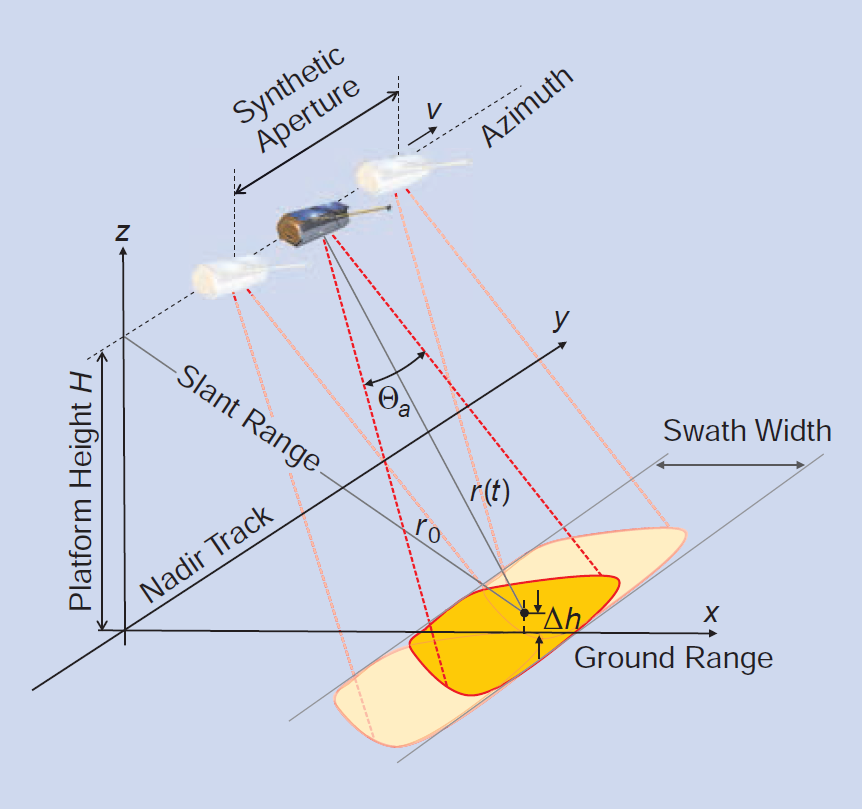
\includegraphics[width=12cm]{Bilder/SAR_Prinzip.png}
    \caption{Prinzip des Synthetic Aperture Radar - Quelle: \cite{tutorial_on_sar}}
    \label{fig:sar_prinzip}
\end{figure}

Die Rauigkeit ist eine Eigenschaft der reflektierenden Oberfläche und hat großen Einfluss auf das reflektierte Signal. Ist diese im Verhältnis zu verwandten
Wellenlänge gering so kommt es zur Spiegelung und nur ein geringer bis kein Anteil des kehrt zum Empfänger zurück. Doch auch die Form und Exposition der Oberfläche nimmt 
Einfluss auf das reflektierte Signal. So werden Flächen unterschiedlich stark bestrahlt. Ist eine dem System abgewandte Fläche steiler geneigt als der Depressionswinkel 
liegen Sie sogar im Radarschatten und werden gar nicht bestrahlt \cite{einfuehrung_in_fernerkundung}. Im Gegensatz zu optischen Aufnahmeverfahren liefern die Rohdaten 
einer Befliegung mit Radarsensoren noch keine Bilddaten. Um Bilder zu erzeugen, bedarf es zunächst einer komplexen Verarbeitung. Dabei werden die Daten entlang des Azimuts und der Blickrichtung gefiltert. 
In der Regel repräsentieren die Pixelwerte eines aus Radardaten abgeleiteten Bildes der Reflektivität der korrespondierenden Fläche. 
Mittels Geocodierung kann das so entstandene Bild verortet werden. Zusätzlich können diverse Kalibrierungen vorgenommen werden. Dazu gehören Verfahren welche Rauscheffekte 
minimieren, die geometrischen Eigenschaften verbessern oder die Interpretation der Bilder erleichtern \cite{tutorial_on_sar}. 

\subsection{Copernicus Programm}
\subsubsection{Ziele}
\subsubsection{Sentinel 1}
\subsubsection{Datenzugang}
\subsection{Überschwemmungsmonitoring}
\subsection{Schnittstellen}
\subsection{OGC und OGC Standards}
\subsection{OGC API - Processes - Part 1: Core}
\subsubsection{Ziele}
\subsubsection{Aufbau}
\subsection{Evaluationskriterien}

